\documentclass[15pt,letterpaper]{article}

\PassOptionsToPackage{hyphens}{url}

\usepackage{setspace}
\doublespacing
\usepackage[]{natbib}
\bibliographystyle{apalike}
% \bibliographystyle{plainnat}

% === MARGINS ===
\addtolength{\hoffset}{-0.75in} 
\addtolength{\voffset}{-1.25in}
\addtolength{\textwidth}{1.5in} 
\addtolength{\textheight}{2.25in}

% == ENVS ==
\newenvironment{tightcenter}{%
  \setlength\topsep{0pt}
  \setlength\parskip{0pt}
  \begin{center}
}{
  \end{center}
}

% == PACKS ==
\usepackage{color,soul}
\usepackage{graphicx} % to use pngs in tex (include graphix)
\usepackage{calc} % To scale \pagewidth with \real{float}
\usepackage{pgfplots} % To draw histogram

\pgfplotsset{
  compat=1.17, 
colormap/viridis
} % request specific version of pgfplots

\usepackage{calc} % to use \real for text -> numeric
\usepackage{pgf} % to store numeric variables
\usepackage{subcaption} % to place two figures horizontally
\usepackage{caption} % to refer subfigure
\renewcommand{\thesubfigure}{(\alph{subfigure})}
\captionsetup[sub]{labelformat=simple}
\captionsetup[table]{font={stretch=1.2}}  % adjust line space in captions of TABLE and FIGURES
\captionsetup[figure]{font={stretch=1.2}}  


\usepackage{tikz}
\usetikzlibrary{automata,positioning}
\usetikzlibrary{arrows.meta, positioning, automata}
\usetikzlibrary{spy}
\usetikzlibrary{shadows}
\usetikzlibrary{arrows,positioning,shapes.geometric} % for dnn flowchart


\tikzset{
  font={\fontsize{10pt}{0}\selectfont}}
\usepackage{forest}
\tikzset{
  Decision/.style = {%
    draw,
    line width=1.4pt
  },
  Lottery/.style = {%
    draw,
    line width=1.4pt
  },
  Outcome/.style = {%
    circle,
    minimum width=3pt,
    fill,
    inner sep=0pt
  }
}
\usepackage{csquotes}
\usepackage{lipsum}
\usetikzlibrary{arrows.meta,automata,positioning} % to draw directed-weighted-graph


\usepackage{amsmath, amssymb, latexsym} % NN
\usepackage{tikz}% NN
\usetikzlibrary{decorations.pathreplacing}% NN
\usetikzlibrary{fadings}% NN


\usepackage{xltabular}
\usepackage{booktabs}

\usepackage[breakable, skins]{tcolorbox} % to add factual asepct inside a frame

\usepackage[title]{appendix}

%to prevent page and footnotes swalloen by the table


% == Checkmarks == 
\usepackage{bbding}
\usepackage{pifont}
\usepackage{wasysym}
\usepackage{amssymb}
% ================

% == BIBS ==
% \usepackage{natbib}

\usepackage{diagbox}

\usepackage[bottom]{footmisc}

\usepackage[
  hidelinks,
  pdftex, 
  bookmarksopen=true, 
  bookmarksnumbered=true,
  pdfstartview=FitH, 
  breaklinks=true, 
  urlbordercolor={0 1 0}, 
  citebordercolor={0 0 1}]
  {hyperref}

\usepackage[ruled,vlined,linesnumbered]{algorithm2e}
\SetKwFor{For}{for (}{) $\lbrace$}{$\rbrace$}

%%% Coloring the comment as blue
\newcommand\mycommfont[1]{\footnotesize\ttfamily\textcolor{blue}{#1}}
\SetCommentSty{mycommfont}

\SetKwInput{KwInput}{Input}                % Set the Input
\SetKwInput{KwOutput}{Output}   
\usepackage{algpseudocode}% http://ctan.org/pkg/algorithmicx
\usepackage{varwidth}% http://ctan.org/pkg/varwidth


\usepackage{titlesec}

\setcounter{secnumdepth}{4}

\titleformat{\paragraph}
{\normalfont\normalsize\bfseries}{\theparagraph}{1em}{}
\titlespacing*{\paragraph}
{0pt}{3.25ex plus 1ex minus .2ex}{1.5ex plus .2ex}


% == SPACES == 

% == CMMDS ==
\newcommand{\tit}{
\Large \bf
Analyzing the Investment Behavior of Congressmen Using Graph Neural Networks: A Study on Identifying the Primary Sources of Investments
}
\newcommand\spacingset[1]{\renewcommand{\baselinestretch}
{#1}\small\normalsize}

% To draw embedding layer
\newcommand*{\xMin}{0}%
\newcommand*{\xMax}{6}%
\newcommand*{\yMin}{0}%
\newcommand*{\yMax}{9}%
% To draw conv output
\newcommand*{\xMinOut}{10}%
\newcommand*{\xMaxOut}{11}%
\newcommand*{\yMinOut}{1}%
\newcommand*{\yMaxOut}{8}%


% == VARS == 
\pgfmathsetmacro{\heatmap}{1}

\makeatletter
\setlength{\@fptop}{0pt}
\makeatother

% == START (PageCounter, Mode)
\begin{document}

\spacingset{1.25}

\setcounter{page}{0}
\vspace{-.1in}

% == TITLE (includes DraftDate)
{\title{
    \tit
  }
  \author{
    Suyeol Yun
  \thanks{Department of Political Science, MIT. Email: \href{mailto:syyun@mit.edu}{syyun@mit.edu}\\
  % **The reproducible code and data can be found at the following link: \href{https://github.com/syyunn/efd}{https://github.com/syyunn/efd}.
  }
  }
  \maketitle
}

\thispagestyle{empty}
\vspace{-.1in}

% \begin{abstract}
%   This paper addresses the limitations of previous research on congressional investment, which only measured excess returns without specifying which types of congressional knowledge explained the behavior. The goal of this study is to reveal whether privileged knowledge acquired from their congressional role influences their stock trading behavior. To achieve this, a predictive analysis using a Graph Neural Network was performed to determine how a social network composed of committees, bills, and companies, and their interactions, can predict the trading patterns of congressmen. The study used graph data that captures the influence of committees on companies, using lobbying data to show which companies lobby for which bills and which committees have jurisdiction over them. This research examines how political network information can reveal the previously unknown relationship between corporate lobbying, committee jurisdiction over bills, and congressmen's stock trading. The paper concludes that this research provides a more detailed visual map of information flow, highlighting where congressmen acquire information about companies and how they reflect this knowledge in their stock trading behavior. 
%   % The paper concludes by suggesting that this study will be of interest to political scientists interested in understanding the relationship between political networks and investment behavior.
% \end{abstract}
% \clearpage

% == INTRO ==
\section{Introduction}
\spacingset{2} % gives a slightly more margin between abstract and introduction
The investment behavior of congressmen has always been a topic of interest for researchers as it raises concerns about conflicts of interest, insider trading, and abuse of power. Members of Congress have access to privileged and confidential information, such as pending legislation, government contracts, and upcoming regulations. 
If members of Congress use this information to make investments, it can be seen as unfair and unethical as they have an advantage over other market participants who do not have access to this information. Furthermore, people elect their representatives to Congress to serve the public interest, and not to enrich themselves personally. 
If members of Congress use their positions to gain financial benefits, it can be seen as a breach of public trust and may undermine the integrity of the democratic system.

Although many studies have investigated the investment behavior of congressmen, there are still gaps in the literature. \cite{zi11} and \cite{zi24} found that Senators and House representatives beat the market and enjoy excess returns while \cite{eg13} found that they don't. 
However, the common limitation of current work is that they don't specify the exact source of congressional knowledge and how that knowledge affects their behavior.

% The biggest problem in this line of research is about how to prove they ``do'' invest with which ``privileged knowledge''.
The main issue in this area of research is how to prove that politicians are using their inside knowledge to make investments. Just because they make a lot of money from their investments doesn't necessarily mean they are using privileged information. However, many high-profile cases have linked this knowledge to their committee assignments, sponsoring of bills, or their home state and potential connections to local businesses. Therefore, future research should focus on developing a reliable method to track down the sources of this privileged knowledge that is more closely linked to investments that show abnormally high returns. This will help to identify which politicians are involved in unethical financial practices and how they are doing it.

\section{Preliminary Analysis}\label{prelim}
In my initial research, I analyzed the excess return for each transaction made by Senators with specific stocks, comparing the return on investment to the federal reserve rates. The results, shown in Figure \ref{fig:agg-ex-r}, suggest that Senators do not generally make significant excess returns from their trading, which is consistent with the findings of \cite{eg13}. However, I did find a few outliers who made substantial gains, some of which have been reported by journalists, while others have not been publicly exposed. An important finding from these outliers is that committee information seems to enable some Senators to enjoy unusually high returns from their trading. 
For instance, Senator Ron Wyden from Oregon traded three semiconductor industry stocks, namely AMAT, KLAC, and AVGO, and gained a significant excess return of 170\%, 115\%, and 70\%, respectively (refer to Figure \ref{fig:agg-ex-r}). What stands out is that he bought all three stocks on the same day, April 6, 2020, during a time when the market was falling due to concerns about the pandemic's impact on the economy. He then sold all three stocks on the same day, April 6, 2021, after President Biden proposed a \$50 billion boost to the US chips industry. It is reasonable to assume that Senator Ron Wyden, being the chair of the Senate finance committee, had prior knowledge of this issue before it was made public. This is because the Senate finance committee introduced the bill ``S.3933 - CHIPS for America Act'' after the announcement on June 10, 2020.

As another example, Senator Ron Wyden made a 38\% ROI from his investment in an American wine producing company (Constellation Brand, Inc. - Ticker: STZ) when the Trump administration imposed additional tariffs on wines imported from Europe.
Since the Senate finance committee has jurisdiction over trade, it is reasonable to assume that Senator Ron Wyden had prior knowledge of this issue before it was made public.

In addition, David Perdue, a former senator from Georgia, obtained an estimated excess return of 10\% from his investment in BWX Technologies Inc., a company that supplies nuclear components to the US Navy. What is notable is that he made consecutive purchases of the stock that turned into sales after he was named chairman of the Senate Armed Services Subcommittee on Seapower.

\begin{figure}[h]
  \centering
  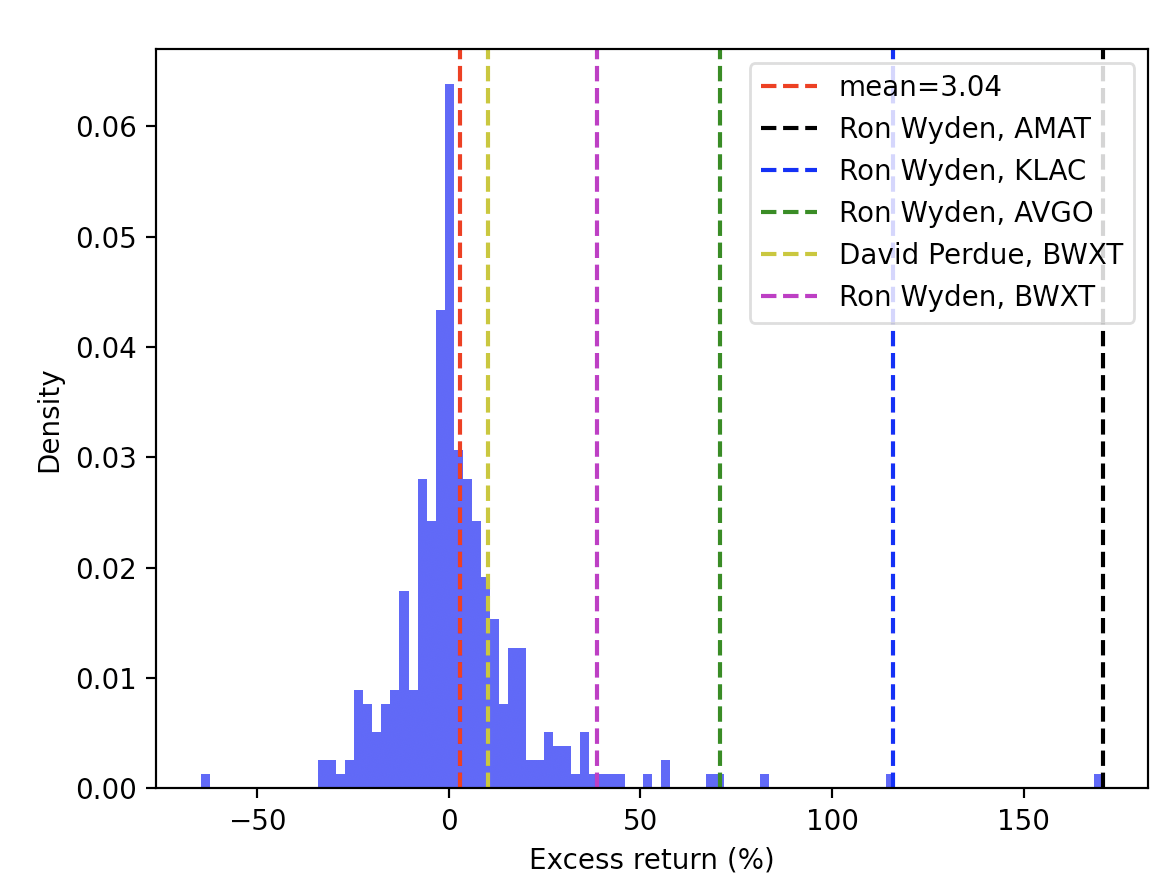
\includegraphics[width=1\textwidth]{imgs/ex-r/aggregate.png}
  \caption{Distribution of mean of each distribution of excess return for $333$ distinct pairs of (Senator, Ticker).}
  \label{fig:agg-ex-r}
\end{figure}

\begin{figure}[h]
  \centering
  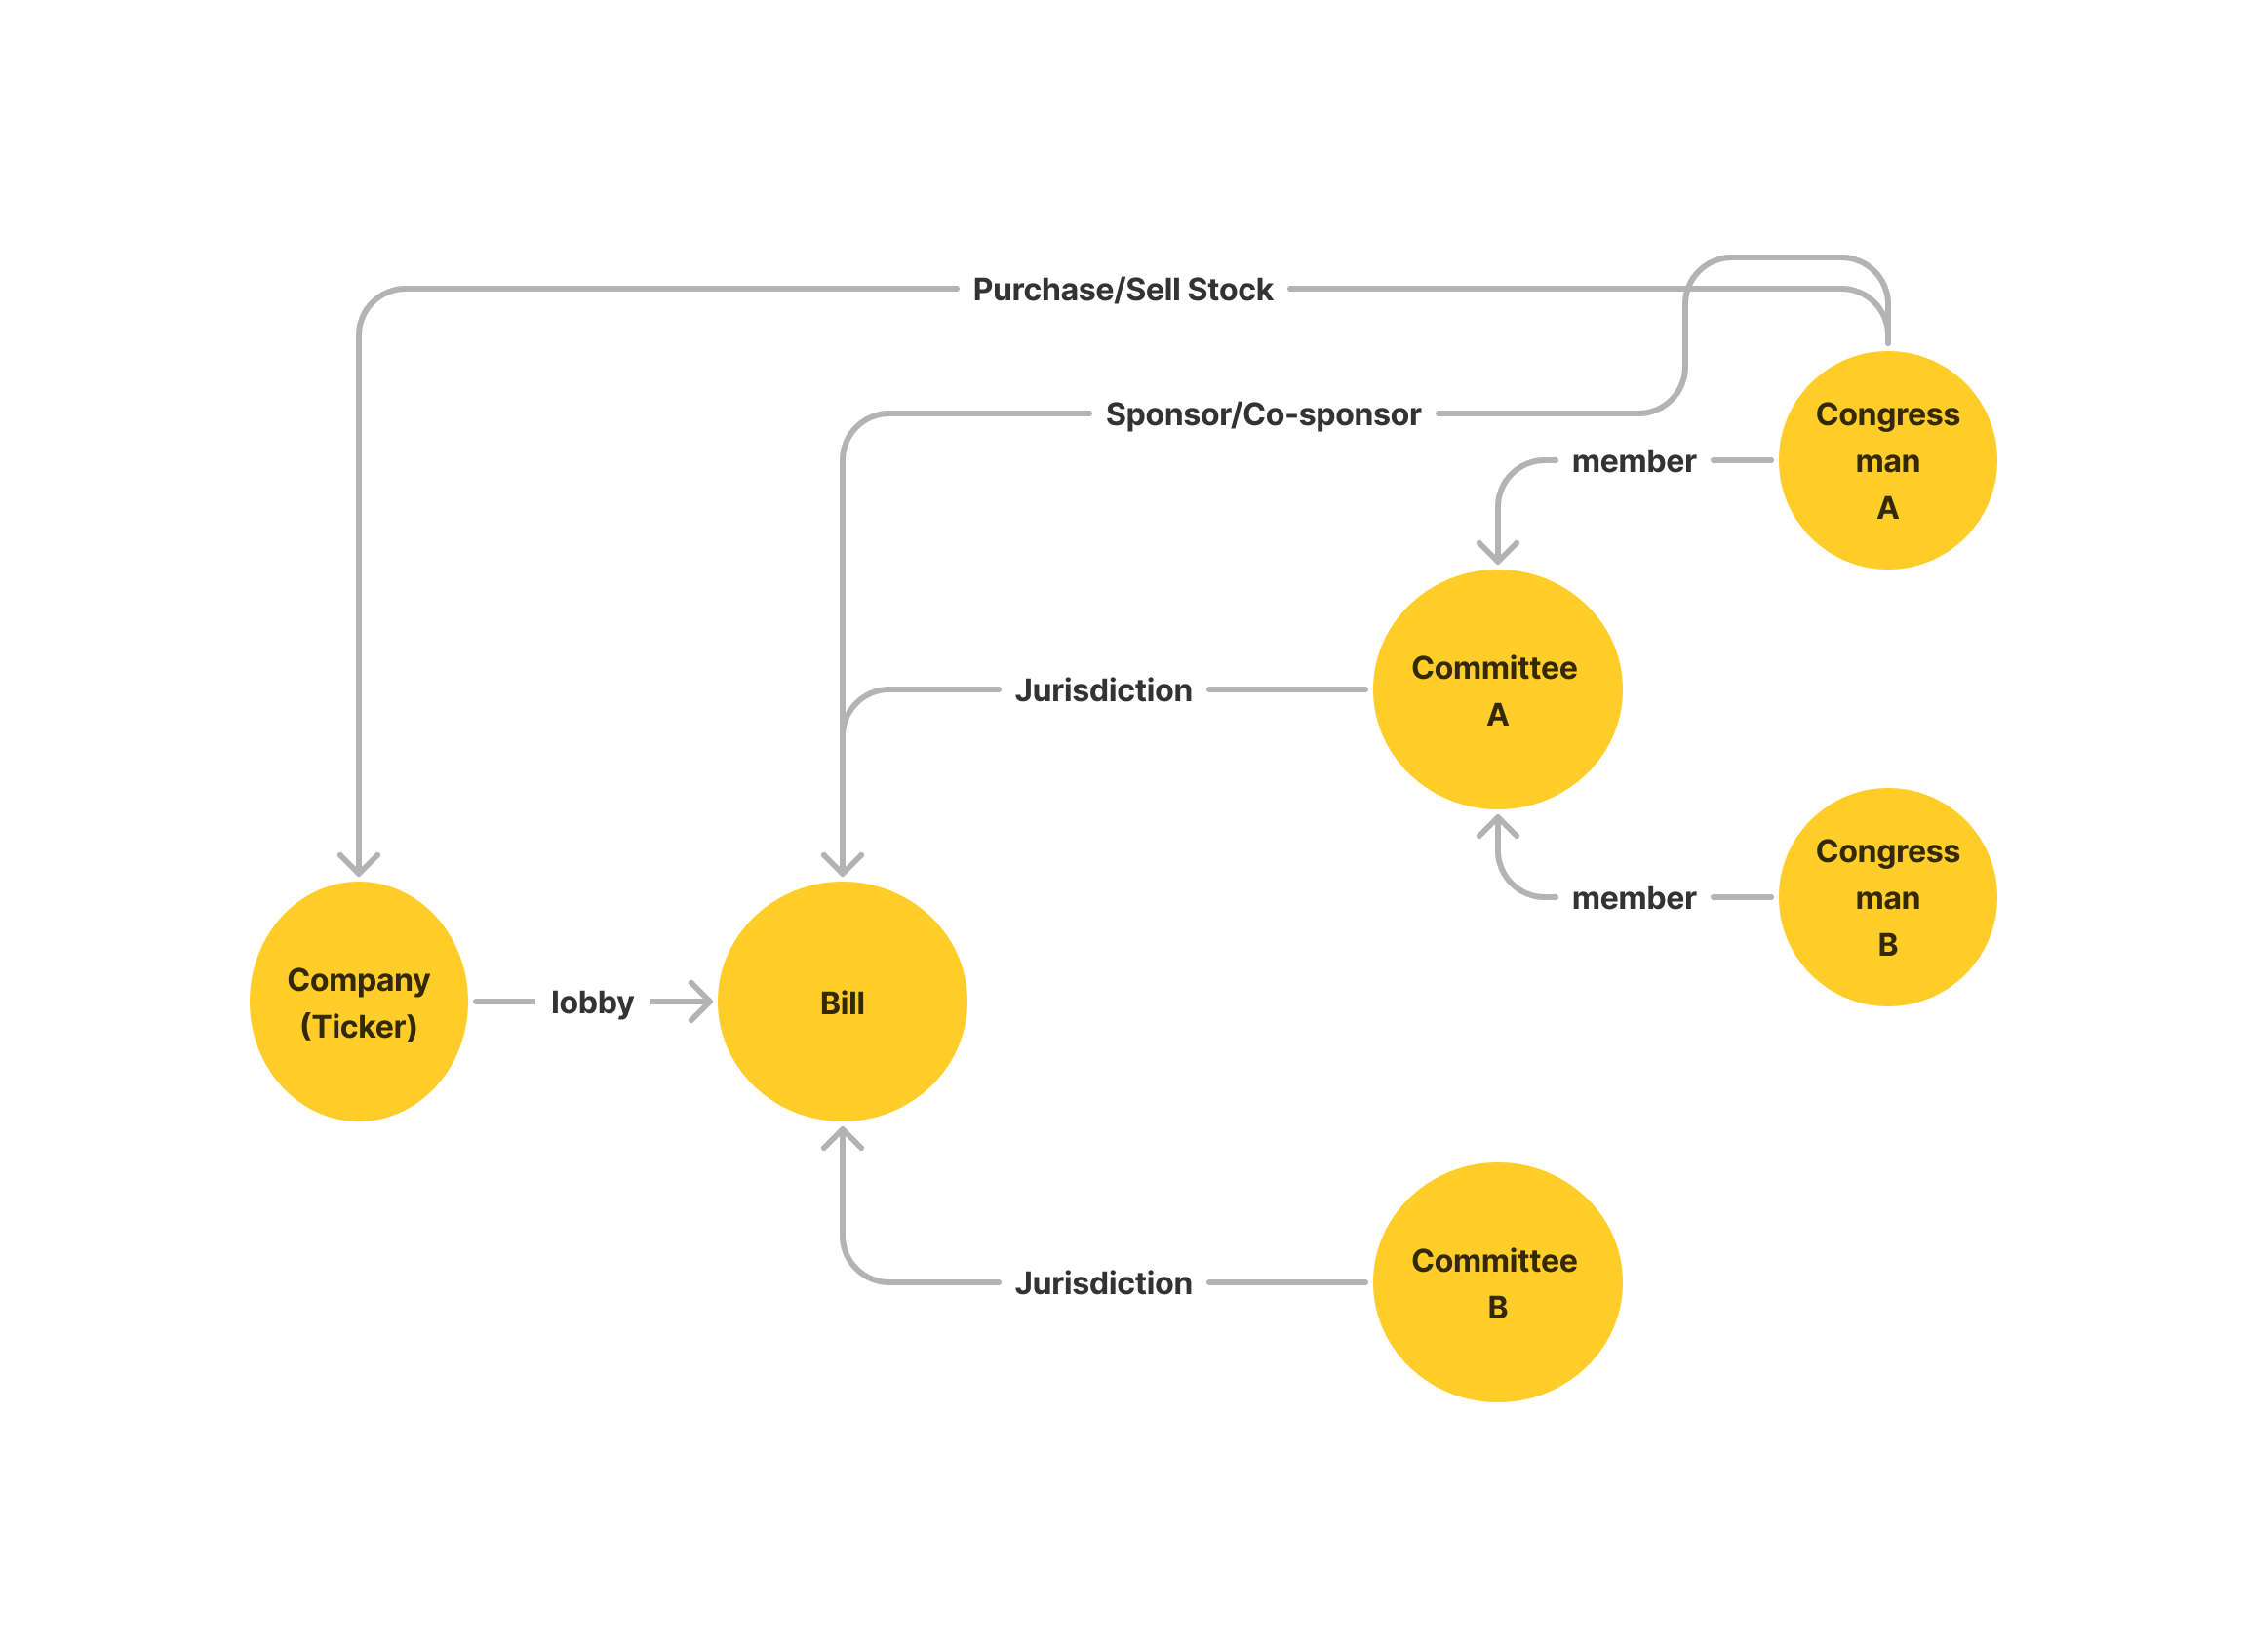
\includegraphics[width=1\textwidth]{imgs/cgd.png}
  \caption{Interaction graph between committees, bills, companies, and congressmen in congressional investment.}
  \label{fig:cbd}
\end{figure}


\section{Data and Methodology}
After analyzing the initial results, I have decided to investigate how committee membership impacts the trading behavior of Congressmen. Typically, each Congressmen is assigned to one or two committees, which are responsible for overseeing the legislation on a specific topic or bill. Companies that have a stake in the legislation have varying levels of interest and involvement, and this relationship is illustrated in Figure 2.

If the Lobbyview data is merged with my transaction data, it would be able to capture the interactions between bills, committees, companies, and Congressmen. Since these interactions can be represented as structured graph data, I plan to use a Graph Neural Network (GNN) for predictive analysis. The GNN will predict a Congressmen's investment in a specific stock using a graph network that includes information on bills, companies lobbying on those bills, committees with jurisdiction over those bills, and the Congressmen assigned to those committees.

A Graph Neural Network (GNN) is a type of neural network that can analyze graph-structured data. The main reason for using GNN in our research is because the data we are analyzing has a graph structure, representing different types of entities interacting with each other. Unlike traditional tabular data, graph data has a unique structure that requires a special type of model to process it. GNN can leverage the benefits of neural networks to encode complex patterns and dependencies in the graph data to effectively predict the quantity of interest, in our case the probability of stock trading of Congressmen. GNNs are also suitable for large-scale data analysis as the network involve a massive amount of data, with over 200,000 bills and 70,000 companies represented as nodes and their interactions as edges. GNNs can efficiently process such large-scale data by analyzing localized neighborhoods around each node.

Task-wise, I plan to use a Graph Neural Network (GNN) to perform a link prediction task. The input data will be a graph consisting of bills, companies, committees, and congressmen. The aim of the link prediction task is to predict which stock transactions are most likely to occur for a given congressman based on the interactions between these entities represented as a graph.

In addition, to make the GNN more interpretable, I will use a GNNExplainer \citep{gnne}, which will identify a subgraph that maximizes the mutual information with the GNN's prediction. 
Using the GNNExplainer will make the prediction task more interpretable, allowing us to understand how specific interactions between certain entities in the graph are likely to affect the prediction of stock transactions.
For example, for the prediction of Ron Wyden's semiconductor stock trading introduced in Section \ref{prelim}, I would expect GNNExplainer to provide a list of companies lobbied for CHIPS for America Act, like Samsung Electronics, Apple, Applied Materials, TSMC, QUALCOMM, Microsoft, Intel along with his committee memebership to the Senate Finance Committee as the ground of this prediction.
This information would help us understand why Ron Wyden made such trade.

\section{Conclusion}
The current literature lacks research on the specific information sources that lead to congressmen's stock transactions. Therefore, my research goal is to address this gap by identifying the source of information that instigated these transactions. To achieve this, I plan to merge the stock transaction data I collected with lobbyview data, which will allow me to capture the level of importance of committees to companies with lobbying activities.

Currently, I am merging this data and planning to use GNN for predictive analysis. However, before proceeding with deep learning using GNN, I am interested in knowing if there are other commonly used methods by political scientists to predict something with graph-structured data input. For my research, I will be using network data as input to predict each congressperson's stock trading activity.

Furthermore, I am seeking feedback on whether there are any ``causal-like'' estimands that can help achieve my research goal of identifying the primary source of information that congresspeople use. Currently, my approach using GNN with GNNEXplainer is purely predictive analysis and lacks a causal approach in a statistical sense. If there are any causal estimands that can help me achieve my goal, I would like to explore those avenues.

I have shared this research proposal with Insong, who agrees with my motivation and method. He is familiar with GNN as he has been working on a project using GNN with KAIST for over a year. I would like to know if this research direction would be persuasive for a political science paper in general.

Additionally, I am open to any straightforward advice to improve my research proposal. I am still in the early stages of my research, and I would appreciate any feedback to help me refine my approach. Please do not hesitate to share your thoughts.



\bibliography{biblo.bib}
\end{document}